\setchapterstyle{lines}
\labch{appendix}
\renewcommand{\thefootnote}{\arabic{footnote}}


% =======================================
% === START RASPBERRY PI ICSP CHAPTER ===
% ======================================= 


\pagelayout{wide} % Remove margins
\chapter{Syllabus} \labch{syllabus}

\section*{Course Description} \labsec{course_desc}
This course is intended to give students exposure to practical electronic design and grant them additional programming experience. 
All of this will be accomplished through the lens of developing an instrumentation package that can be deployed as a project and capture/record data. 
Students will use basic Arduino learning kits to cultivate their interests. 
Graduate students taking the course will be required to follow more industry-related programming practices for the Arduino programming, will be held to a higher product quality standard, and will be required to develop a more advanced instrumentation package than the undergraduates. 
Course lectures will be supplemented by weekly (or as weekly as possible) demonstrations using real measurement equipment used by the Ocean Engineering department.

    \subsection*{Meeting Times}
        \subsubsection*{Lectures}
        Monday, Wednesday, Friday; 16:00-16:50 (0h50min)\\
        Fall 2022, August 22 - December 9\\
        Room TBD

        \subsubsection*{Office Hours}
        Monday, Wednesday, Friday; 13:00-15:00\\
        Or, by appointment (preferred)\\
        Link 155 or Frueauff 100

    \subsection*{Objectives \& Outcomes}
    The goal of this course is the provide a basic instruction on practical electrical engineering and computer programming through the lens of instrumentation design. 
    After introducing and refreshing basic concepts like electrical components, digital electronics, and C++ basics, students will be taught how industry professionals make real-world measurements using various instruments. At the end of the course, students will be able to:
    \begin{enumerate}
        \item Understand how various measurement devices capture, record, and transmit information to researchers and engineers
        \item Have a fundamental knowledge of programming Arduino-based microcontrollers
        \item Have a fundamental knowledge of Printed Circuit Board design, manufacture, and assembly
        \item Apply the fundamental concepts learned in lecture and through demonstrations on a practical Individual Course Project.
    \end{enumerate}

    \subsection*{Target Audience \& Prerequisites}
    On the undergraduate side, this course is intended for students who do not have a basic familiarity with basic electronics and programming with Arduino. 
    The ELEGOO Arduino Starter Kit recommended for this class has supplementary information that will assist students in understanding exactly what is occurring with various projects. 
    Students are strongly encouraged to delve deeper into the topics covered in class and pursue a challenging Individual Course Project. 
    Individuals with a strong drive to learn independently will benefit greatly during this course.

    On the graduate side, this course is designed for students who have a basic knowledge of electronics and programming with Arduino or C++. 
    Embedded design experience is also desired as it will be most beneficial during the Individual Course Project. 
    While the ELEGOO Arduino Starter Kit will give the basics, graduate students will be expected to expand upon the projects covered in the kit and use more sophisticated programming techniques. 
    The Individual Course Project will also need to be well considered and adequately demonstrate the student's knowledge and motivation to learn outside the classroom.

    \subsection*{Course Resources}
    The course material will be regularly updated on Canvas and \href{https://github.com/Legohead259/OCE4531-Material} {GitHub}. The GitHub repository will have all of the supplementary and study material required by students. The Canvas page may also contain these files, but GitHub will be the most up to date.
    
    Students will be \emph{required} to purchase their own Arduino learning kit for this course. They can be easily found on Amazon.
    \begin{enumerate}
        \item \href{https://www.amazon.com/ELEGOO-Project-Tutorial-Controller-Projects/dp/B01D8KOZF4}
        {UNO R3 Super Starter Kit - \$34}
        \item \href{https://www.amazon.com/EL-KIT-001-Project-Complete-Starter-Tutorial/dp/B01CZTLHGE} 
        {UNO R3 Complete Starter Kit - \$60}
        \item \href{https://www.amazon.com/EL-KIT-008-Project-Complete-Ultimate-TUTORIAL/dp/B01EWNUUUA}
        {Mega R3 Complete Ultimate Starter Kit - \$55}
    \end{enumerate}

    Graduate students will also be required to order a Raspberry Pi - or equivalent Single Board Computer (SBC), for this course. 
    It is strongly recommended to purchase a Raspberry Pi 400 Full Computer Kit (\href{https://www.adafruit.com/product/4796}{Adafruit}) with an accompanying T-Cobbler GPIO Breakout (\href{https://www.adafruit.com/product/2028}{Adafruit}).
    
    Due to the recent chip shortage, Raspberry Pis may be hard to find or prohibitively expensive. If students are unable to acquire their own Raspberry Pis or similar SBCs, they may ask for a loaner unit from the instructor. \textbf{Please note that if the loaner unit is \emph{not} returned by the end of the semester, the student will be given an ``Incomplete'' grade until the instructor has been given the device.}

\section*{Grading Policies}
This course covers several student performance metrics: (i) assignments, (ii) participation, (iii) midterm exam, and (iv) an Individual Course Project. The weighting for this metrics is below:
\begin{table*}[ht!]
    \begin{tabular}{c | c}
        \toprule
        Metric                      & Weight \\

        \midrule
        Assignments                 & 20\% \\
        Participation               & 10\% \\
        Midterm Exam                & 30\% \\
        Individual Course Project   & 40\% \\

        \bottomrule
    \end{tabular}
\end{table*}

Students will be assigned the following letter grade and GPA quality points based on their weighted sum assignment scores according to:

\begin{table*}[h!]
    \begin{tabular}{c | c | c}
        \toprule
        Score & Letter Grade & Quality Points \\
        
        \midrule
        90-100              & A     & 4 \\
        80-89               & B     & 3 \\
        70-79               & C     & 2 \\
        60-69\footnotemark  & D     & 1 \\
        <60                 & F     & 0 \\

        \bottomrule
    \end{tabular}
\end{table*}
\footnotetext{Undergraduate students only. \textbf{Graduate students will fail below a 70.}}

\section*{Course Schedule}
\begin{table*}[h!]
    \begin{tabular}{ c | c | c | c }
        \toprule
        Week & Monday & Wednesday & Friday \\

        \midrule
        1   & Syllabus, setup       & Binary and boolean logic          & Project discussion    \\
        2   & Digital logic         & Digital logic                     & YSI Castaway demo     \\    
        3   & \textbf{NO CLASS}     & Multiplexers, registers, states   & HOBO meter demo       \\
        4   & ADC Conversion        & Communication methods             & Survey gear demo      \\
        5   & Electrical comps      & Simple circuit debugging          & Launchsonde demo      \\
        6   & Intro to Fusion 360   & ECAD-Schematics                   & Lowell/Thetis demo    \\
        7   & ECAD-Schematics       & ECAD-PCB basics                   & Sidescan SONAR demo   \\
        8   & \textbf{NO CLASS}     & Inertial Measurement Units        & Midterm exam          \\
        9   & Sensor Fusion         & AHRS design                       & CODAR system demo     \\
        10  & Distance sensors      & Environmental sensors             & Soldering workshop    \\
        11  & Analog filtering      & Digital filtering                 & Remote sensing demo   \\
        12  & Gerber gen. and order & PCB manufacture techniques        & \textbf{NO CLASS}     \\
        13  & PCB assembly (hand)   & PCB assembly (PnP)                & Robotics demo         \\
        14  & Buffer day            & \textbf{NO CLASS}                 & \textbf{NO CLASS}     \\
        15  & Data transmission     & Power considerations              & Work day              \\
        16  & ICP Presentations     & ICP Presentations                 & ICP Presentations     \\

        \bottomrule
    \end{tabular}
\end{table*}

\section*{Assignment Schedule} \labsec{assignment_sch}

\begin{table*}[h!]
    \begin{tabular}{ c | c }
        \toprule
        Assignment & Due Date \\

        \midrule
        Get Arduino Kit, Raspberry Pi\footnotemark  & August 26     \\
        RGB LED                                     & August 29     \\
        Digital inputs and interrupts               & September 5   \\
        Active buzzer                               & September 12  \\
        Servo control, ICP proposal\footnotemark[2] & September 19  \\
        Ultrasonic sensor module                    & September 26  \\
        DHT temperature sensor                      & October 3     \\
        Midterm Exam                                & October 14    \\
        ICP schematic                               & October 24    \\
        ICP PCB design                              & November 11   \\
        Assembled ICP PCB                           & November 28   \\
        Final ICP presentation                      & December 5    \\
        Final ICP report                            & December 12   \\

        \bottomrule
    \end{tabular}
\end{table*}
\footnotetext[2]{\textbf{Graduate Students \emph{Only}}}

\section*{Other Important Dates}

\begin{table*}[h!]
    \begin{tabular}{ c | c }
        \toprule
        Event & Date \\

        \midrule
        Last day to drop without a "W"  & August 31 \\
        Last day to drop with a "W"     & October 31 \\

        \bottomrule
    \end{tabular}
\end{table*}

\section*{Course Policies} \labsec{course_policies}

    \subsection*{Online Course Management}

    This course will be published in the online learning tool, \href{instructure.fit.edu}{Canvas}, and will be made readily available to all students. 
    Canvas provides an online cross-platform solution for students and instructors to engage and will handle all of the assignment submissions and \emph{preliminary} grades for students.
    Assignments will be issued and submitted through the Canvas platform and students will be expected to submit the required documents by the due date and time listed on the assignment submission box.
    If, for whatever reason, assignments are unable to be turned in through Canvas, they must be emailed to the instructor and timestamped by the date and time established.
    
    Grades will also be posted on Canvas for students to track their progress in status in the course.
    However, there is no guarantee that the posted grade in Canvas will represent the final course grade submitted to the registrar, nor may it be up-to-date if grade corrections are necessary.
    In the event a student is not satisfied by their grade posted in Canvas, they are more than welcome to schedule a \emph{face-to-face} meeting with the instructor to discuss.
    Emailed requests to change grades may be considered but it will be more effective to meet with the instructor in-person to ensure the change is made properly.

    Canvas will also have a "Files" section where students can find relevant course resources and documents to aid in their studies.
    Students may request certain documents be uploaded to Canvas to share with their classmates and they may download all files freely if they wish to have their own local copies.
    The Canvas may be periodically updated to reflect changes or addendums to course content, but it may not necessarily reflect the most up-to-date information.
    For the most updated course material, please consult the class \href{https://github.com/OCE4531-Materials}{GitHub Repository}. \emph{You may be surprised what you find in there...}

    \subsection*{Weekly Projects}

    For the first couple of weeks of the course, students will be expected to put their Arduino starter kits to use with various projects.
    These are intended to slowly ramp up in complexity and give students a glimpse of what practical electronics and programming looks like.
    Projects will be due by 23:59 Eastern Time on the day specified in the \hyperref[sec:assignment_sch]{Assignment Schedule} section.
    
    \paragraph*{Late Policy} Submissions for assignments will be accepted up to the date of the students ICP presentation.
    However, for every day (24 hours) after the deadline, starting the minute after the deadline passes, 10 points will be deducted from the assignment down to an absolute maximum of 50\%.


    \subsection*{Individual Course Project}

    The Individual Course Project (ICP) is designed to encompass all of the elements taught throughout the course into a single package.
    Undergraduate students will be tasked with taking one of the Arduino projects available in their starter kits and converting it to an Arduino-compatible shield.
    Essentially, taking the circuit they already made on a breadboard, drawing the schematic in an ECAD software like Fusion 360, routing the PCB in the same software, and order and assembling the final PCB. 
    Students will be tasked with writing up their ICP in a comprehensive report and giving a quick final presentation at the end of the semester.

    \paragraph*{Financial Policy} Students will be required to purchase their PCBs and any additional components for their ICP not already available to them in their Arduino kits or by the Underwater Technology Lab. 
    Currently, each student is expected to pay around \$5 for the PCB order and most undergraduate students should be using components already present in their Arduino kits. 
    The final amount each student will have to pay for their PCB will be determined at the time of ordering by the instructor.
    
    Sponsorship by the UTL may be requested and may be granted on a case-by-case basis. Students with ICPs that prove useful to the lab's operation may have their fees waived depending on several external factors.
    This will be determined by the time of ordering.
    Students wishing to be sponsored should contact the instructor ASAP for details.

    \paragraph*{Failure Policy} \emph{FAILURE IS AN OPTION.} It is well-understood that students may have a non-functional ICP at the end of the semester. \textbf{That is okay!}
    The university environment is about learning and especially learning while failing.
    Therefore, students who do not have a functional PCB have two options for recourse:
    \begin{enumerate}
        \item they may explain, in copious detail, what the failure on the PCB was and how it would be addressed in the next revision, were it to be manufactured. 
        \item they will have until December 12 to submit a fixed PCB that is working, but may have "bodges" or other modifications
    \end{enumerate}
    If students elect for Option 1, they will receive penalty points on their ICP. These points will be subjectively detracted according to the instructor. As a general guideline, \emph{the simpler the mistake, the harsher the penalty will be}. 
    For instance, a missing connection in the schematic or trace on the PCB will have more points deducted than two components not talking due to EMI or other nuanced electrical engineering problem.
    \emph{Attention to detail is important!}

    \paragraph*{Late Policy} Late submissions on any part of the ICP will not be tolerated. For every 24 hours after the minute an ICP-related assignment is due, 10\% will be deducted from the \textbf{overall} ICP grade.
    Simply put, if four ICP-related assignments are turned in a minute late, then the student will receive a 0\% overall for their ICP weight category.
    
    Additionally, students who do not submit a PCB gerber package by the order deadline (November 11) may end up forfeiting their potential grades.
    This deadline is in place to ensure ample time for PCB assembly and testing and all orders will be placed at the same time.
    If a student does not submit the PCB gerber package by the deadline, the onus and financial responsibility will be on them to order the PCBs in a timely manner such that they can still assemble and test their ICP.

    \subsection*{For Students with Handicaps and/or Disabilities}
    Students with handicaps and/or disabilities will be given special considerations depending on their condition and Florida Tech policy. Please meet with the instructor privately to discuss any concerns or arrangements. 

    \subsection*{Academic Dishonesty Policy}
    Students who are caught cheating or plagiarizing will be given an audience with the instructor to discuss the situation. 
    Some cases are simple mistakes or coincidences with no ill-intent and can be rectified with a penalty to the assignment grade.
    Severe cases of rampant cheating or plagiarism \emph{with} ill-intent or severe negligence will be referred to the Dean of Students in accordance with academic policy present in the Florida Tech handbook.
    Students who are referred to the Dean of Students may forfeit their overall grades for the course and may face academic probation, suspension, or expulsion from Florida Tech - as the Dean determines.
    
    Academic Dishonesty incidents will not be considered until the assignment is officially submitted. 
    Therefore, students are strongly encouraged to meet with the instructor with questions about if a portion of their assignment could be considered academically dishonest.

    \subsection*{Title IX}
    Title IX of the Educational Amendments Act of 1972 is the federal law prohibiting discrimination based on sex under any education program and/or activity operated by an institution receiving and/or benefiting from federal financial assistance. Behaviors that can be considered “sexual discrimination” include sexual assault, sexual harassment, stalking, relationship abuse (dating violence and domestic violence), sexual misconduct, and gender discrimination. You are encouraged to report these behaviors. 

    \paragraph*{Reporting} Florida Tech can better support students in trouble if we know about what is happening.  Reporting also helps us to identify patterns that might arise - for example, if more than one complainant reports having been assaulted or harassed by the same individual.

    \subsection*{Regarding Unusual or Extraneous Circumstances}
    \emph{``If anything can go wrong, it will'' - Murphy's Law}

    It is well-understood that incidents will occur in this fickle thing we call life.
    Students and instructors alike are human and we cannot predict what will happen in the next five minutes let alone the next few days.
    In the event of something unexpected or unusual, please contact the instructor ASAP.
    Each case will be considered for its severity, impact on student well-being, and impact to the student's education.
    Some unforeseen circumstances may warrant an extension to an assignment deadline, a reschedule of a test, or other remedies depending on its severity.
    
    Conversely, the instructor may have incidents where class may need to be cancelled or an assignment delayed. The instructor reserves the right to maneuver the class as they see fit, but it would not be possible without the participation of the students.
    If the instructor is late to class, please allow for up to 15 minutes before departing.
    If the instructor needs to cancel a class, there will be an announcement made through the Canvas page, ideally, well ahead of the class start time.
    Additionally, the instructor may elect to hold class in a remote session through Zoom, should that be a necessary option.
    
    Students, please try to be flexible and understanding, and the instructors will do the same.

\pagelayout{margins} % Restore margins


% =======================================
% === START RASPBERRY PI ICSP CHAPTER ===
% ======================================= 


\pagelayout{wide} % Remove margins
\chapter{In-Circuit Serial Programming Guide}

Microcontrollers are special embedded processors that are capable of executing specific code with a high efficiency.
They are used throughout the world in various devices ranging from handheld gaming devices, medical units, military 
hardware, and digital signage. Recently, the Arduino foundation made playing with microcontrollers easier as they
created a platform where users could write code, plug in a microcontroller over USB, flash the chip, and see the results
- nearly in real-time. They helped usher in the Maker Renaissance we found ourselves in today, by obfuscating the more
complex tasks in microcontroller programming using high-level software and other microcontrollers.

The purpose of this guide is to help de-obfuscate low-level microcontroller programming by showing you what is really happening when you give the "Upload" command in the Arduino IDE.

\section*{What is In-Circuit Serial Programming?}

In-Circuit Serial Programming (ICSP) is the fundamental way to program a microcontroller. Microcontrollers typically
store their programs on SPI flash memory which can be read or written over as the programmer demands. By temporarily 
disabling the microcontroller and overwriting the contents of the SPI flash memory, we can reprogram the microcontroller
with different code.

On the Arduino boards, when you upload code over USB, a secondary microcontroller on the board interprets the USB
communications and translates them to the UART serial protocol. The bootloader on the main microcontroller then uses 
the data coming from the UART bus to reprogram the SPI flash memory, thus reprogramming the Arduino. This is a form of 
ICSP, but adds complexity to both the circuit and fundamental microcontroller firmware. 

A simpler version of ICSP is accessing the SPI flash memory directly. On the Arduino Uno board, the ICSP header is 
easily visible and can be used by any device that has an SPI bus to reprogram the microcontroller. 
If, for instance, the USB-Serial bridge on the board has its program memory corrupted ICSP can be used to re-flash the 
correct firmware onto the chip. Alternatively, if the chip is completely non-functional, the primary microcontroller 
can still be used with new code being deployed over the ICSP pins.

\begin{figure}
    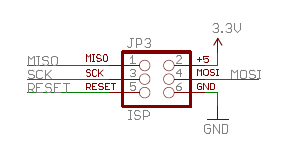
\includegraphics[width=3.5in]{rpi_icsp/icsp-header.png}
    \caption[Arduino ICSP Header]{Pinout of the Arduino Uno and Mega ICSP header}
    \labfig{arduino_icsp_header}
\end{figure}

Note that different microcontrollers may have different implementations of ICSP. Another popular form is the Single
Wire interface. Please refer to your microcontroller's datasheet for specific information.

\section*{Arduino as In-circuit Serial Programmer}

For this example, we will be using an Arduino as an In-circuit Serial Programmer (ISP) to program another Arduino over 
ICSP. The Arduino Foundation provides a sketch in the examples folder of the Arduino IDE to configure an Arduino board 
as an ISP. First, plug in the Arduino Uno to the ICSP header as shown in Figure \ref{fig:arduino_icsp_hookup} and according to Table \ref{tab:arduino_icsp_hookup}. On most boards, there is no reverse-polarity protection, so make sure the 5V and GND wires are plugged in correctly. 

\begin{figure}
    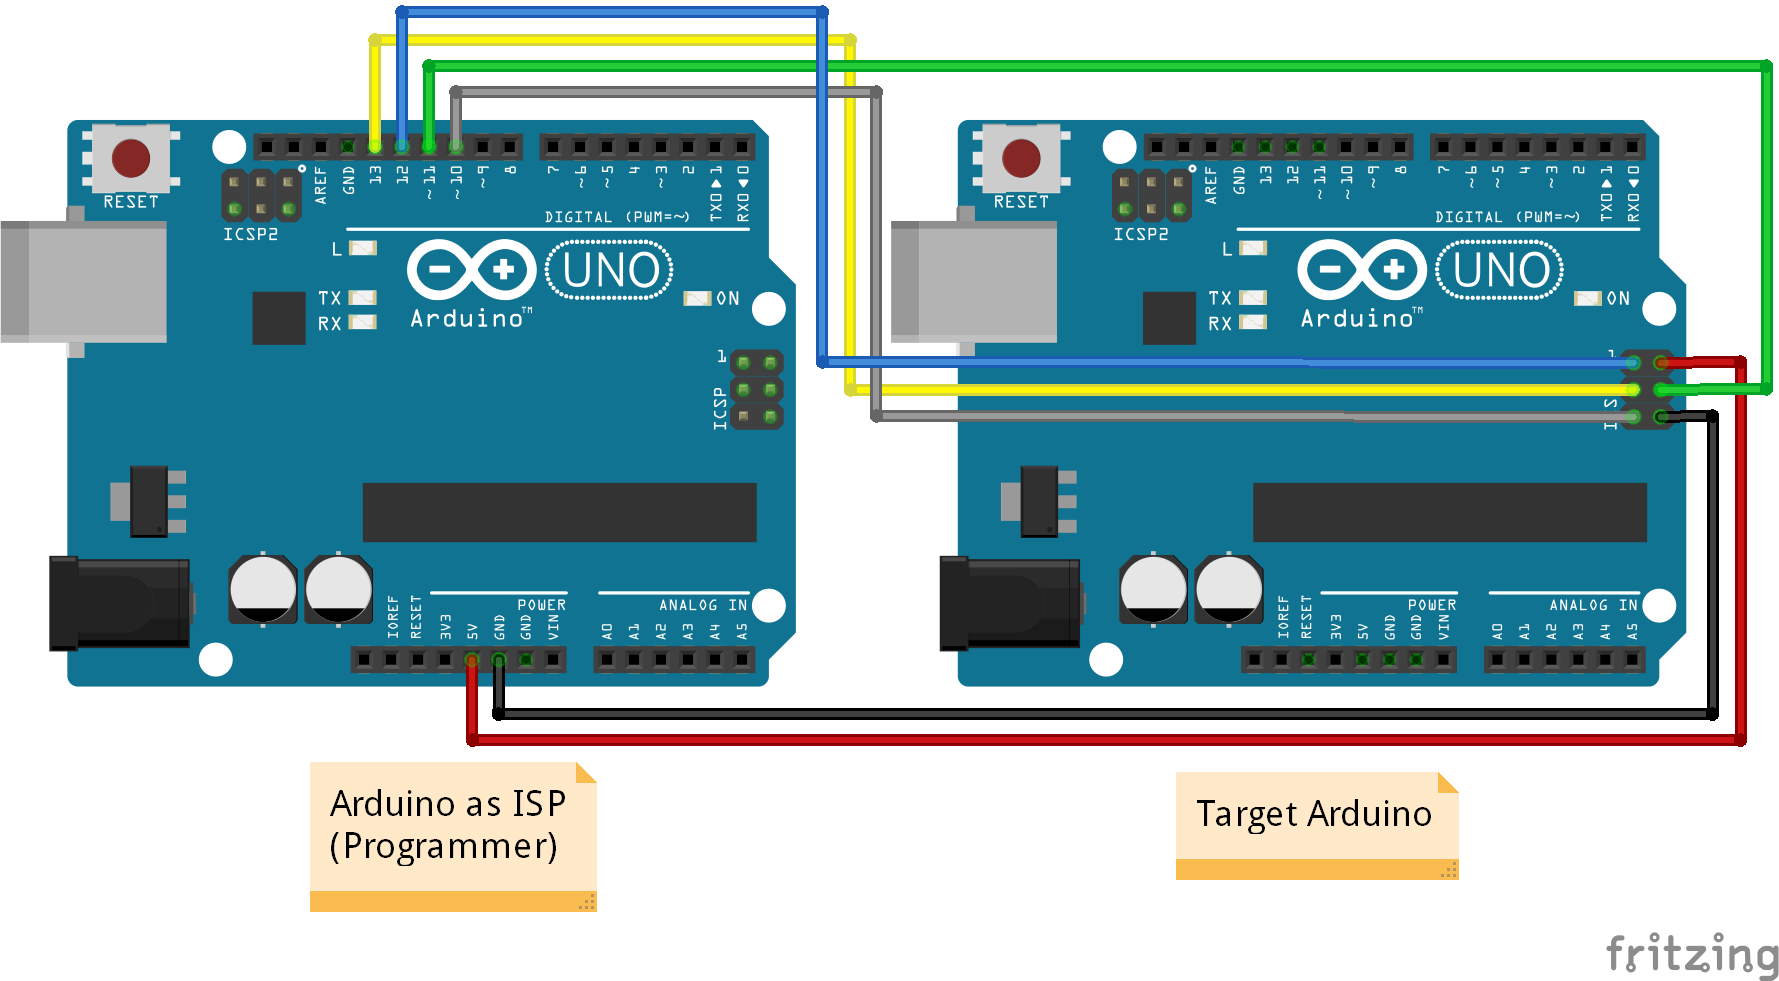
\includegraphics[]{rpi_icsp/Fritzing_ArduinoasISP_AVR_Programmer_bb.png}
    \caption[ArduinoISP Hookup Diagram]{Diagram showing how to hook up an ArduinoISP programmer and Arduino ICSP target.Retrieved from \url{https://learn.sparkfun.com/tutorials/installing-an-arduino-bootloader/hardware-hookup}}
    \labfig{arduino_icsp_hookup}
\end{figure}

\begin{table}[h!]
    \caption[ArduinoISP Hookup Guide]{ArduinoISP hookup table for target and programmer}
    \begin{tabular}{ c | c }
        \toprule
        Programmer & Target \\

        \midrule
        DIO 12  & MISO (Pin 1)  \\
        DIO 13  & SCK (Pin 2)   \\
        DIO 10  & RESET (Pin 3) \\
        5V      & 5V (Pin 4)    \\
        DIO 11  & MOSI (Pin 5)  \\
        GND     & GND (Pin 6)   \\

        \bottomrule
    \end{tabular}
    \labtab{arduino_icsp_hookup}
\end{table}

After wiring up the boards, plug the Arduino Uno into the programming computer. This will apply power to the system and should allow you to program the Uno as you normally would. Then, navigate the ArduinoISP sketch located in the “examples” folder of the Arduino IDE (Figure \ref{fig:arduino_isp_loc}) and upload the sketch to the Arduino Uno.

\begin{figure}
    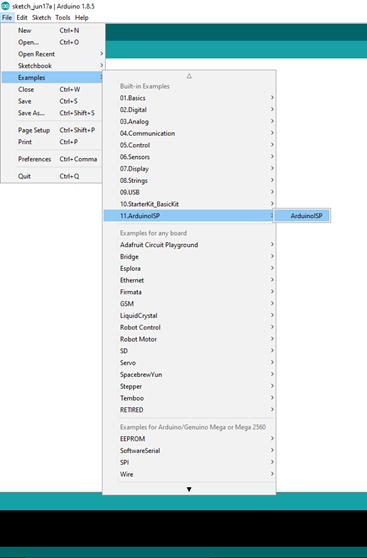
\includegraphics[width=3.5in]{rpi_icsp/ArduinoISP_ss.png}
    \caption[ArduinoISP Example]{Location of ArduinoISP sketch in the Arduino IDE}.
    \labfig{arduino_isp_loc}
\end{figure}

Once the ArduinoISP sketch is uploaded, navigate to a sketch to upload to the target board configuring the compiler to the target board and processor (Figure \ref{fig:arduino_isp_config}). 
Use the same COM port as the Arduino Uno and use the “Upload Using Programmer” option  shown in Figure \ref{fig:arduino_isp_upload}. 
If you get any errors such as “Unable to communicate with device” or “Invalid device signature”, check your wiring and try again.

\begin{figure}
    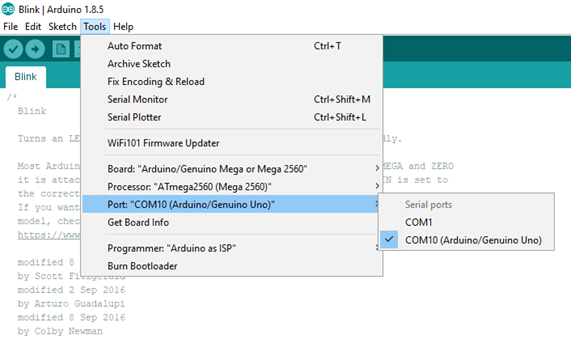
\includegraphics[width=6in]{rpi_icsp/ArduinoISP_config_ss.png}
    \caption[ArduinoISP Config]{Configuring the Arduino IDE to compile for the correct board}.
    \labfig{arduino_isp_config}
\end{figure}

\begin{figure}
    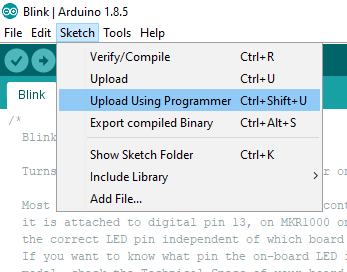
\includegraphics[width=3.5in]{rpi_icsp/ArduinoISP_upload_ss.png}
    \caption[ArduinoISP Upload]{Upload Using Programmer sketch option}.
    \labfig{arduino_isp_upload}
\end{figure}

While this example used the basic Blink example code, this process can be done for any appropriate Arduino sketch onto most Arduino-compatible boards. 
On some embedded devices, a common USB interface may not be accessible and therefore ICSP is the only programming option.

\section*{Using a Raspberry Pi as ISP}

For the graduate portion of this class, we will be using a Raspberry Pi to upload code to the Arduino boards over ICSP. 
The Raspberry Pi uses 3.3V logic levels which are not completely compatible with the 5V logic levels of the Arduino board.
Therefore, it is strongly recommended to use a breadboard to breakout the Raspberry Pi's pins to a logic level converter
and connect it from there to the Arduino's ICSP header. Please refer to Figure \ref{fig:rpi_icsp_bb} for hookup information. 
The pinout for this configuration can be found in the figure, which we will use later with AVRDUDE

    \begin{figure}[h!]
        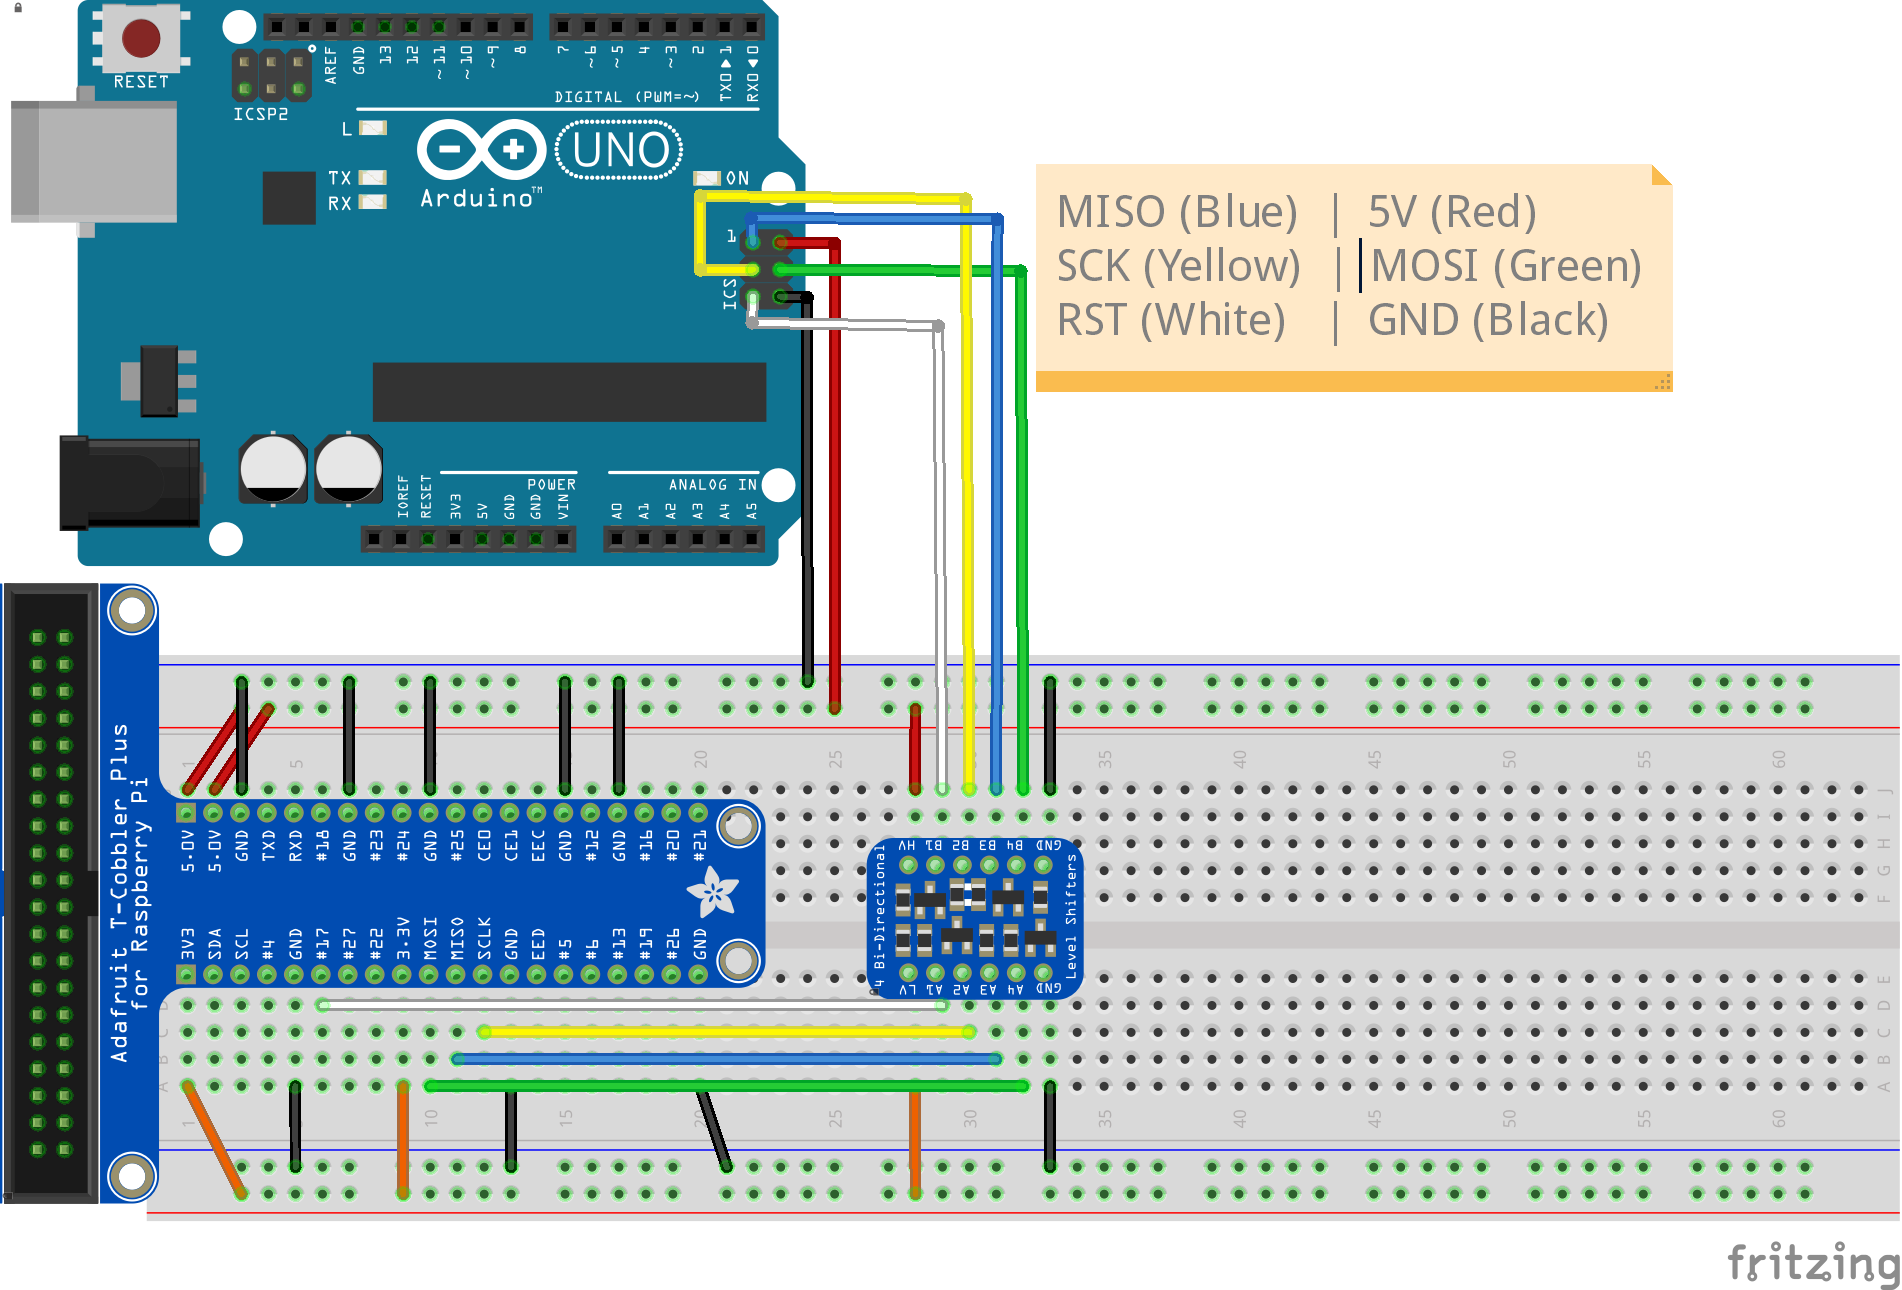
\includegraphics[width=5in]{rpi_icsp/rpi_icsp_bb.png}
        \caption[Raspberry Pi ISP Breadboard]{A wiring diagram of how the Raspberry Pi should be connected to the Arduino ICSP headers through a breadboard and a \href{https://www.adafruit.com/product/757}{logic-level     converter}. 
        Created using Fritzing \url{https://fritzing.org}}.
        \labfig{rpi_icsp_bb}
    \end{figure}

    \begin{table}[h!]
        \caption[RaspberryPi as ISP Hookup Guide]{Raspberry Pi as ISP hookup table for target and programmer}
        \begin{tabular}{ l | c | c }
            \toprule
            Programmer & Logic Level Converter & Target \\
    
            \midrule
            3V3                                 & LV    & NC\footnotemark   \\
            NC\footnotemark[\value{footnote}]   & HV    & 5V                \\
            GPIO 17                             & A1/B1 & RESET             \\
            GPIO 11 (SCLK)                      & A2/B2 & SCK               \\
            GPIO 9 (MISO)                       & A3/B3 & MISO              \\
            GPIO 10 (MOSI)                      & A4/B4 & MOSI              \\
            GND                                 & GND   & GND               \\
    
            \bottomrule
        \end{tabular}
        \labtab{rpi_icsp_hookup}
    \end{table}
    \footnotetext{Not connected}

    \subsection*{Setting up AVRDUDE}
    AVRDUDE is the software package that will upload machine binary to the microcontroller's program storage. 
    The following steps will assume you have already set up the Raspberry Pi with RaspberryPiOS and updated the latest packages. 
    Through this example, we will be operating inside a command terminal through a remote secure login shell, but this process can be repeated inside the command terminal of a headed set up.

    First, in the open terminal execute the following command:

    \begin{lstlisting}[style=kaolstplain,linewidth=1.5\textwidth]
        sudo apt-get install avrdude
    \end{lstlisting}

    This will install AVRDUDE on the Raspberry Pi so we can flash .hex files onto the microcontroller. To verify the installation, execute:

    \begin{lstlisting}[style=kaolstplain,linewidth=1.5\textwidth]
        avrdude -v
    \end{lstlisting}

    If the output is something like:

    \begin{lstlisting}[style=kaolstplain,linewidth=1.5\textwidth]
        avrdude: Version 6.3-20171130
            Copyright (c) 2000-2005 Brian Dean, http://www.bdmicro.com/
            Copyright (c) 2007-2014 Joerg Wunsch

            System wide configuration file is "/etc/avrdude.conf"
            User configuration file is "/home/pi/.avrduderc"
            User configuration file does not exist or is not a regular file, skipping

        avrdude: no programmer has been specified on the command line or the config file
            Specify a programmer using the -c option and try again
    \end{lstlisting}

    Then the installation is good and AVRDUDE has created a user configuration file that we can edit. To begin this process, execute the following commands in the terminal:

    \begin{lstlisting}[style=kaolstplain,linewidth=1.5\textwidth]
        cp /etc/avrdude.conf ~/avrdude_gpio.conf
    \end{lstlisting}

    \begin{lstlisting}[style=kaolstplain,linewidth=1.5\textwidth]
        nano ~/avrdude_gpio.conf
    \end{lstlisting}

    The first command copies the default AVRDUDE configuration file to a new file in the home directory of user. The second command will open this file in the Nano file editor, pulling up a screen like Figure \ref{fig:avrdude_gpio_config_nano}.
    
    \begin{figure}[h!]
        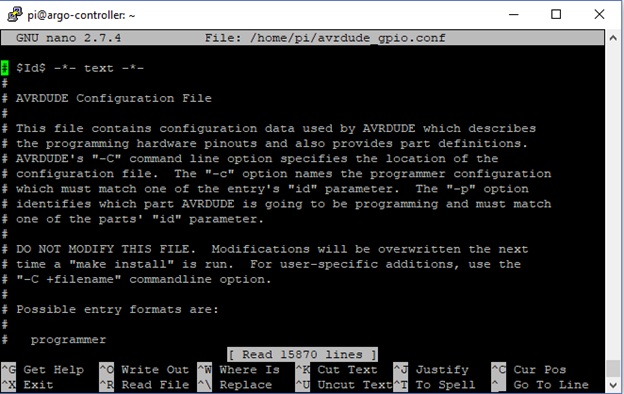
\includegraphics[]{rpi_icsp/avrdude_gpio_conf_nano_ss.png}
        \caption[AVRDUDE GPIO config file open in Nano]{The top of the avrdude\_gpio.conf file in Nano}
        \labfig{avrdude_gpio_config_nano}
    \end{figure}

    Once in the file, press CTRL\+\_, then CTRL\+V to navigate to the bottom of the file. There, paste the following block of code:

    \begin{lstlisting}[style=kaolstplain,linewidth=1.5\textwidth]
        programmer
            id = "gpio_icsp";
            desc = "Use the Linux sysfs interface to bitbang GPIO lines for programming the Arduino;
            type = "linuxgpio";
            reset = 17;
            sck = 11;
            mosi = 10;
            miso = 9;
        ;
    \end{lstlisting}

    This creates an AVRDUDE programmer that uses the GPIO pins specified in Table \ref{tab:rpi_icsp_hookup} to program the Arduino over ICSP. Press CTRL+X then Y then ENTER to save and exit the file; the AVRDUDE programming tool is now configured.

    \subsection*{Preparing a Sketch for ICSP Uploading (Arduino)}

    Once you have a sketch ready for the microcontroller to run, configure the compiler for your board, same as Figure \ref{fig:arduino_isp_config}.
    Select the ``Export compiled Binary'' option in the Arduino IDE (Figure \ref{fig:arduino_ide_export}). 
    This will create two files in the sketch`s directory, both ending with ``.hex'', but one will have ``.with\_bootloader'' in the middle. 
    The file we want to upload is the one without the bootloader, highlighted in Figure \ref{fig:arduino_sketch_folder}. \footnotemark
    
    \footnotetext{This will disable the USB programming bootloader. This will need to be re-flashed with the bootloader if you want to upload code to the microcontroller via USB again.}
    
    \begin{figure}[h!]
        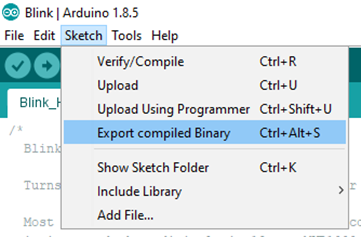
\includegraphics[width=3.5in]{rpi_icsp/arduino_export_binary_ss.png}
        \caption{Arduino IDE ``Export compiled Binary'' option}
        \labfig{arduino_ide_export}
    \end{figure}

    \begin{figure}[h!]
        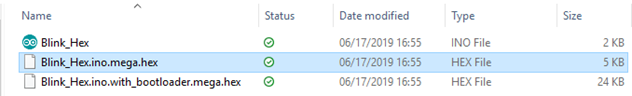
\includegraphics[]{rpi_icsp/arduino_binary_folder_ss.png}
        \caption{The sketch and its compiled binaries in their folder}
        \labfig{arduino_sketch_folder}
    \end{figure}

    \subsection*{Preparing a Sketch for ICSP Uploading (VS Code)}

    This part assumes you have already initialized the Arduino development environment within VS Code.
    In VS Code, open the ``arduino.json'' file in the /.vscode folder of your workspace. Add the following line to the bottom of the file:

    \begin{lstlisting}[style=kaolstplain,linewidth=1.5\textwidth]
        "output": ".arduinobuild"
    \end{lstlisting}

    This will create a new folder in the root directory of the workspace called ``.arduinobuild'' that will hold all of pre-compiled binaries for your Arduino sketch, logs, and other things that are not important right now.
    Inside this folder will be two files: ``[sketch\_name].ino.bin'' and ``[sketch\_name].bootloader.bin''.
    As before, the one we want to upload is the one without the bootloader.\footnotemark[1]

    \subsection*{Programming the Microcontroller}

    Transfer the binary file to the Raspberry Pi using your preferred method of choice.
    This is most easily done over a USB stick or a File Transfer Protocol like Secure Copy.
    Applications like \href{https://winscp.net/eng/download.php}{WinSCP} make this process easy for beginners.
    Place the file in a working destination directory - ideally, a project folder you have already set up beforehand.
    Then, open a terminal on the Raspberry Pi and execute the following command:
    
    \begin{lstlisting}[style=kaolstplain,linewidth=1.5\textwidth]
        sudo avrdude -p [Microcontroller] -C ~/avrdude_gpio.conf -c gpio_icsp -v
    \end{lstlisting}

    Note: the \textbf{[Microcontroller]} in this command needs to be replaced with the name of the microcontroller in use (e.g. ``atmega328p'' for the Arduino Uno or ``atmega2560'' for the Arduino Mega).

    This will verify that the Raspberry Pi can talk to the microcontroller and verifies that the chip is operating nominally.

    If there are any issues, make sure you are executing this command with ``sudo'' and that the configuration file matches with the GPIO pins used in the schematic; check the wiring connections to the Arduino; and check that the file path for ``avrdude\_gpio.conf'' is correct .\footnote{The "\textasciitilde" in the file path only denotes the relative directory you are currently in. If the file is NOT in the same directory that you are executing the command in, you must put the path in lieu of the “\textasciitilde ”.}

    Once you have established communications with the Arduino, execute:

    \begin{lstlisting}[style=kaolstplain,linewidth=1.5\textwidth]
        sudo avrdude -p [Microcontroller] -C ~/avrdude_gpio.conf -c gpio_icsp -v -U flash:w:[filename]:i
    \end{lstlisting}

    Where again \textbf{[Microcontroller]} needs to be replaced with the name of the microcontroller and \textbf{[filename]} needs to be replaced with the path and name of the binary sketch file you copied to the Raspberry Pi.
    The end of a successful write should look something like this:

    \begin{lstlisting}[style=kaolstplain,linewidth=1.5\textwidth]
        avrdude: AVR device initialized and ready to accept instructions

        Reading | ################################################## | 100% 0.00s

        avrdude: Device signature = 0x1e9801 (probably m2560)
        avrdude: safemode: lfuse reads as FF
        avrdude: safemode: hfuse reads as D8
        avrdude: safemode: efuse reads as FD
        avrdude: NOTE: "flash" memory has been specified, an erase cycle will be performed
                To disable this feature, specify the -D option.
        avrdude: erasing chip
        avrdude: reading input file "Blink_Hex.ino.mega.hex"
        avrdude: writing flash (1462 bytes):

        Writing | ################################################## | 100% 0.41s

        avrdude: 1462 bytes of flash written
        avrdude: verifying flash memory against Blink_Hex.ino.mega.hex:
        avrdude: load data flash data from input file Blink_Hex.ino.mega.hex:
        avrdude: input file Blink_Hex.ino.mega.hex contains 1462 bytes
        avrdude: reading on-chip flash data:

        Reading | ################################################## | 100% 0.82s

        avrdude: verifying ...
        avrdude: 1462 bytes of flash verified

        avrdude: safemode: lfuse reads as FF
        avrdude: safemode: hfuse reads as D8
        avrdude: safemode: efuse reads as FD
        avrdude: safemode: Fuses OK (E:FD, H:D8, L:FF)

        avrdude done.  Thank you.
    \end{lstlisting}

    If there is an error (most commonly with a file name) it will likely occur after the first reading block. 
    The -v argument of the command gives error statements in the output so you can error trace and find the problem. 
\pagelayout{margins} % Restore margins